\chapter{Theoretical Fundamentals} % Chapter title

\label{chapter:theoretical_fundamentals} % For referencing the chapter elsewhere, use \ref{chapter:computational_neuro} 

\def \blochwidth {0.4}
\def \qspherewidth {0.5}
\def \histogramwidth {0.4}
\newcommand{\bloch}{\emph{Bloch}-Sphere}
\newcommand{\qsphere}{Q-Sphere}
\newcommand{\hgate}{$\mathrm{H}$-Gate}

\newcommand{\xgate}{$\mathrm{X}$-Gate}
\newcommand{\ygate}{$\mathrm{Y}$-Gate}
\newcommand{\zgate}{$\mathrm{Z}$-Gate}

\newcommand{\rygate}{$\mathrm{RY}$-Gate}
\newcommand{\rxgate}{$\mathrm{RX}$-Gate}
\newcommand{\rzgate}{$\mathrm{RZ}$-Gate}

\newcommand{\crygate}{$\mathrm{CRY}$-Gate}
\newcommand{\crxgate}{$\mathrm{CRX}$-Gate}
\newcommand{\crzgate}{$\mathrm{CRZ}$-Gate}

\newcommand{\cxgate}{$\mathrm{CX}$-Gate}
\newcommand{\cygate}{$\mathrm{CY}$-Gate}
\newcommand{\czgate}{$\mathrm{CZ}$-Gate}

\newcommand{\frenchquotes}[1]{«~#1~»}

%----------------------------------------------------------------------------------------
\section{Quantum Computing}
Classical computing consist of 1's and 0's and have for years shaped the computational world and progress. Quantum computing is, from afar, similar. We have \emph{qubits}, which are synonymous to classical \emph{bits}, but are fundamentally different. Whereas a bit can only exist in state 0 or 1, a qubit allows the usage of any state, be it 0, 1 or a mix of those. Such a mix is referred to as a \emph{superposition}\cite{gudder_superposition_1970}. The catch comes when we want to read the value it represents: one cannot directly know the probabilities of measuring 1 or 0 in a qubit, as demonstrated in figure \ref{figure:comparison_bit_qubit_measurement}.

\begin{figure}[!h]
    \centering
    \tikzset{every picture/.style={line width=0.75pt}} %set default line width to 0.75pt        
    
    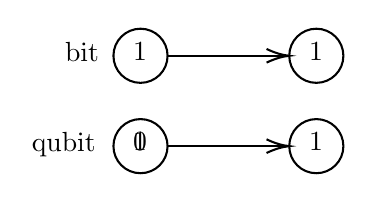
\begin{tikzpicture}[x=0.75pt,y=0.75pt,yscale=-1,xscale=1]
    %uncomment if require: \path (0,300); %set diagram left start at 0, and has height of 300
    % Text Node
    \draw    (117.29, 130) circle [x radius= 13.04, y radius= 13.04]   ;
    \draw (112.29,122) node [anchor=north west][inner sep=0.75pt]   [align=left] {1};
    % Text Node
    \draw    (202, 130) circle [x radius= 13.04, y radius= 13.04]   ;
    \draw (197,122) node [anchor=north west][inner sep=0.75pt]   [align=left] {1};
    % Text Node
    \draw    (202, 173.54) circle [x radius= 13.04, y radius= 13.04]   ;
    \draw (197,165.54) node [anchor=north west][inner sep=0.75pt]   [align=left] {1};
    % Text Node
    \draw (112.29,165.54) node [anchor=north west][inner sep=0.75pt]   [align=left] {0};
    % Text Node
    \draw    (117.29, 173.54) circle [x radius= 13.04, y radius= 13.04]   ;
    \draw (112.29,165.54) node [anchor=north west][inner sep=0.75pt]   [align=left] {1};
    % Text Node
    \draw (79.43,122) node [anchor=north west][inner sep=0.75pt]   [align=left] {bit};
    % Text Node
    \draw (63.43,165.54) node [anchor=north west][inner sep=0.75pt]   [align=left] {qubit};
    % Connection
    \draw    (130.32,173.54) -- (186.96,173.54) ;
    \draw [shift={(188.96,173.54)}, rotate = 180] [color={rgb, 255:red, 0; green, 0; blue, 0 }  ][line width=0.75]    (10.93,-3.29) .. controls (6.95,-1.4) and (3.31,-0.3) .. (0,0) .. controls (3.31,0.3) and (6.95,1.4) .. (10.93,3.29)   ;
    % Connection
    \draw    (130.32,130) -- (186.96,130) ;
    \draw [shift={(188.96,130)}, rotate = 180] [color={rgb, 255:red, 0; green, 0; blue, 0 }  ][line width=0.75]    (10.93,-3.29) .. controls (6.95,-1.4) and (3.31,-0.3) .. (0,0) .. controls (3.31,0.3) and (6.95,1.4) .. (10.93,3.29)   ;
    
    \end{tikzpicture}
    \caption{A comparison of measuring a single bit and a qubit. When measuring the bit, we get the same value that the bit is set to. When measuring a qubit, there is a certain probability of it being 0 and 1, so we measure one of both but don't know the real, internal state of the qubit.}
    \label{figure:comparison_bit_qubit_measurement}
\end{figure}

When measuring a quantum circuit, the qubit states collapse from super positions into the fixed position of 0 or 1. This means that to redo the measurement, the complete circuit has to be rebuilt. After doing multiple measurements on a qubit and collecting the results as shown in table \ref{table:example_counts}, this data can be used to construct a \emph{histogram}\cite{eckstein_lexikon_1994} akin to the one visualized in figure \ref{figure:example_histogram}, out of which one can retrieve the internal probabilities of 1 and 0.

\begin{figure}[!h]
    \begin{subtable}{.5\textwidth}
    \centering
    \begin{tabular}{|c|c|}
         Measured value & Amount  \\
         \hline
         0 & 547 \\
         1 & 987 \\
    \end{tabular}
    \caption{Table containing all measurements done on a qubit in an unknown superposition. The number of occurrences of a measured 1 or 0 is counted and then used to generate the histogram in figure \ref{figure:example_histogram}}
    \label{table:example_counts}
    \end{subtable}
    \begin{subfigure}{.5\textwidth}
        \centering
        \scalebox{\histogramwidth}{
            \includesvg{thesis/Appendices/example_histogram.svg}
        }
        \caption{A histogram generated from the data in table \ref{table:example_counts}, that visually shows the probabilities of 0 and 1. These probabilities can directly be used to understand the superposition of a qubit .}
        \label{figure:example_histogram}
    \end{subfigure}
    \caption{Example of collected measurements from an arbitrary, single qubit, quantum circuit, as well as the corresponding histogram.}
    \label{fig:my_label}
\end{figure}

With these two definitions, the gates used in the quantum circuits of this thesis can be fully 

\newpage

To further understand how a qubit behaves, the very foundations of quantum physics have to be looked at. Postulated by E. Schrödinger in 1925, the \emph{Schrödinger-Equation}\cite{PhysRev.28.1049} gives us the differential equation for the time evolution of a quantum state and their respective solution, shown in equation \ref{equation:schroedinger_time_evolution}, where $H$ denotes a Hamiltonian.

\begin{equation}
    \centering
    \begin{split}
          i\hbar\frac{d}{dt}\psi(t) =\ H\psi(t) \\
        \psi(t) =\ e^{-i\frac{Ht}{\hbar}}\psi(0)
    \end{split}
    \label{equation:schroedinger_time_evolution}
\end{equation}

The expression $U(t) =\ e^-i\frac{Ht}{\hbar}$ itself has the attribute that it is unitary. Through this, the multiplication of $U(t)$ with its conjugate transpose $U(t)^\ast$ results in the identity matrix. This leads to quantum operations being reversible – so-called \emph{bijective functions} - where every output can be reversed to a single input. \par
A mere two years later, Wolfgang Pauli published "Zur Quantenmechanik des magnetischen Elektrons"\cite{pauli_zur_1927}, in which he introduced the \emph{Pauli matrices}. These matrices represent the \emph{spin} of atoms and elementary particles, and are a core element of quantum computing. The definition of these matrices is shown in equation \ref{equation:pauli_matrices}.

\begin{equation}
    \centering
    \begin{split}
        \sigma_x &=\ \begin{pmatrix}0 & 1 \\ 1 & 0\end{pmatrix} =\ \mathrm{X}\\
        \sigma_y &=\ \begin{pmatrix}0 & -i \\ i & 0\end{pmatrix} =\ \mathrm{Y}\\
        \sigma_z &=\ \begin{pmatrix}1 & 0 \\ 0 & -1\end{pmatrix} =\ \mathrm{Z}\\
    \end{split}
    \label{equation:pauli_matrices}
\end{equation}

\newpage

The \bloch\cite{michael_a_nielsen_quantum_2000}, as shown in figure \ref{figure:basic_bloch_sphere}, is used to help visualize quantum operations on a single, \emph{non-entangled}, qubit. The complex \emph{Bloch}-Vector inside the \bloch\ corresponds to the expectation value of measuring a value in a single qubit. To visualize entangled qubits, the \bloch\ by itself is not enough. There are proposed solutions to this problem\cite{gamel_entangled_2016}, which result in a more complex visualization with multiple \bloch s. To solve this issue, IBM created the Q-Sphere\cite{ibm_quantum_visualizations_nodate} as shown in figure \ref{figure:q_sphere_4qubit_h}, which can not only visualize single qubits, but also entangled ones as well as their global phase and probability in form of amplitude.

\begin{figure}[!h]
    \centering
    \begin{subfigure}{.4\textwidth}
        \centering
        \scalebox{\blochwidth}{
            \includesvg{thesis/Appendices/Bloch_Sphere_axis.svg}
        }
        \caption{A basic \bloch\ without any visualized state. The axis $x$ and $y$ are annotated accordingly, but the axis $z$ is annotated with $\ket{0}$ and $\ket{1}$ - the states which are measured and have a corresponding probability assigned to them. The purple arrow shows the \emph{Bloch}-Vector, and currently points to $\ket{0}$, so the state the single qubit is currently in.}
        \label{figure:basic_bloch_sphere}
    \end{subfigure}
    \begin{subfigure}{.4\textwidth}
        \centering
        \scalebox{\qspherewidth}{
            \includesvg{thesis/Appendices/Q_Sphere_State_h_multiqubit.svg}
        }
        \caption{A basic Q-Sphere that shows all possible states of a 4 qubit circuit, as well as the probability of each state, as well as their phase. The probability is encoded into the width of the dots next to the state labels. As all dots are equal, it is clear that all states have the same probability of being measured.}
        \label{figure:q_sphere_4qubit_h}
    \end{subfigure}
    \caption{A comparison of the \bloch\ used to visualize single qubits only, and the Q-Sphere that can visualize multiple qubits.}
    \label{fig:comparison_bloch_sphere_q_sphere}
\end{figure}

When measuring a qubit, the state collapses onto the $z$-axis\cite{feynman_feynman_1965}, which in turn leads to a measurement of either 0 or 1. Initially, all qubits are set to state $\ket{0}$, which is visualized onto the Q-Sphere in figure \ref{figure:state_0_q_sphere}. A circuit that results in said state is visualized in figure \ref{figure:state_0_circuit}, and its mathematical counterpart in equation \ref{equation:state_0_equation}. The states $\ket{\psi_i}$ are used to denote the state of one, or multiple, qubits at the currently marked point of the circuit. These are utilized to mark the states that are calculated throughout this thesis.

\begin{figure}[!h]
    \begin{subfigure}{.5\textwidth}
    \centering
        \scalebox{\qspherewidth}{
            \includesvg{thesis/Appendices/Q_Sphere_State_0.svg}
        }
        \caption{A Q-Sphere with the state $\ket{0}$ visualized onto it.}
        \label{figure:state_0_q_sphere}
    \end{subfigure}
    \begin{subfigure}{.5\textwidth}
    \centering
        \scalebox{1.0}{
        \Qcircuit @C=1.0em @R=1.0em @!R { \\
    	 	\nghost{{q} :  } & \lstick{{q} :  } \barrier[0em]{0} & \qw & \qw & \qw\\
    	 	\nghost{} & \lstick{} & \ket{\psi_0} &\\
    \\ }}
        \caption{A basic circuit consisting of a single qubit $q$ that is initially set to $\ket{0}$. The state vector at point $\ket{\psi_0}$ is shown in equation \ref{equation:state_0_equation}.}
        \label{figure:state_0_circuit}
    \end{subfigure}
    \caption{The circuit with qubit state $\ket{0}$ at position $\ket{\psi_0}$ and its corresponding Q-Sphere visualization.}
    \label{fig:showcase_qubit_state_0_with_circuit}
\end{figure}



\begin{equation}
    \centering
    \begin{split}
        \ket{\psi_0} =\ \begin{pmatrix}1 \\ 0\end{pmatrix} =\ \ket{0}\\
    \end{split}
    \label{equation:state_0_equation}
\end{equation}

\newpage
To create the state $\ket{1}$, the circuit from figure \ref{figure:state_0_circuit} is extended with the Pauli \xgate\cite{qiskit_xgate_nodate}. To verify its behaviour, equation \ref{equation:state_1_equation} takes the state $\ket{\psi_0}$ and multiplies it with the \xgate, which then results in the state $\ket{\psi_1}$, as noted on the circuit \ref{figure:x_circuit}, whilst the figure \ref{figure:state_1_q_sphere} visualizes the state on the Q-Sphere.

\begin{figure}[!h]
    \begin{subfigure}{.5\textwidth}
        \centering
        \scalebox{\blochwidth}{
            \includesvg{thesis/Appendices/Q_Sphere_State_1.svg}
        }
        \caption{The Q-Sphere with the state $\ket{1}$ visualized onto it, which is achieved through the usage of the circuit in figure \ref{figure:x_circuit}}
        \label{figure:state_1_q_sphere}
    \end{subfigure}
    \begin{subfigure}{.5\textwidth}
        \centering\scalebox{1.0}{
        \Qcircuit @C=1.0em @R=0.2em @!R { \\
    	 	\nghost{{q} :  } & \lstick{{q} :  } \barrier[0em]{0} & \qw & \gate{\mathrm{X}} \barrier[0em]{0} & \qw & \qw & \qw\\
    	 	\nghost{} & \lstick{} & \ket{\psi_0} & & \ket{\psi_1} &\\
    \\ }}
        \caption{The circuit from figure \ref{figure:state_0_circuit} extended with a \xgate\ to transform the initial state $\ket{0}$ at position $\ket{\psi_0}$, into the state $\ket{1}$ at position $\ket{\psi_1}$}
        \label{figure:x_circuit}
    \end{subfigure}
    \caption{Caption}
    \label{fig:my_label}
\end{figure}

\begin{equation}
    \centering
    \begin{split}
        \ket{\psi_1} =\ \mathrm{X}\ket{\psi_0} =\ \begin{pmatrix} 0 & 1\\ 1 & 0\end{pmatrix}\begin{pmatrix}1 \\ 0\end{pmatrix} =\ \begin{pmatrix}0 \\ 1 \end{pmatrix}\\
    \end{split}
    \label{equation:state_1_equation}
\end{equation}

As shown in equation \ref{equation:pauli_matrices}, there exist two more Pauli matrices. Like the \xgate\ that corresponds to the Pauli matrix $\sigma_x$, the gates \ygate\cite{qiskit_ygate_nodate} and \zgate\cite{qiskit_zgate_nodate} correspond to the Pauli matrices $\sigma_y$ and $\sigma_z$.
\newpage
To achieve an equal probability of the states $\ket{0}$ and $\ket{1}$, the \emph{Hadamard}-Gate, or \hgate\cite{qiskit_hgate_nodate}, can be used to correctly set up the qubit with one gate. Without it, one would have to use a combination of different gates to achieve the result\cite{voorhoede_hadamard_nodate}, for example $\mathrm{XY}^{\frac{1}{2}}$.


\begin{figure}[!h]
    \begin{subfigure}{.5\textwidth}
        \centering
        \scalebox{\blochwidth}{
            \includesvg{thesis/Appendices/Q_Sphere_State_h.svg}
        }
        \caption{A basic \qsphere\ with the state $\frac{1}{\sqrt{2}}\left(\ket{0} + \ket{1}\right)$ visualized onto it. The equal probability of both states is visualized through the blue dots, which have the same size.}
        \label{figure:state_h_q_sphere}
    \end{subfigure}
    \begin{subfigure}{.5\textwidth}
        \centering\scalebox{1.0}{
        \Qcircuit @C=1.0em @R=0.2em @!R { \\
    	 	\nghost{{q} :  } & \lstick{{q} :  } \barrier[0em]{0} & \qw & \gate{\mathrm{H}} \barrier[0em]{0} & \qw & \qw & \qw\\
    	 	\nghost{} & \lstick{} & \ket{\psi_0} & & \ket{\psi_1} &\\
    \\ }}
        \caption{A simple circuit with one qubit, that is transformed
    through the usage of a \hgate\ to turn the initial state $\ket{0}$ at position $\ket{\psi_0}$ into the state $\ket{1}$ at position $\ket{\psi_1}$. The calculation is shown in equation \ref{equation:equal_superposition_equation}.}
        \label{figure:h_circuit}
    \end{subfigure}
    \caption{A single qubit is set into an equal superposition shown on the \qsphere\ \ref{figure:state_h_q_sphere} generated using the circuit \ref{figure:h_circuit}}
    \label{figure:_one_qubit_h_state_circuit_qsphere}
\end{figure}



\begin{equation}
    \centering
    \begin{split}
        \ket{\psi_1} =\ \mathrm{H}\ket{\psi_0} =\ \frac{1}{\sqrt{2}}\begin{pmatrix} 1 & 1 \\ 1 & -1 \end{pmatrix}\begin{pmatrix}1 \\ 0\end{pmatrix} =\ \frac{1}{\sqrt{2}}\begin{pmatrix}1 \\ 0 \end{pmatrix} + \frac{1}{\sqrt{2}}\begin{pmatrix}0 \\ 1 \end{pmatrix}\\
    \end{split}
    \label{equation:equal_superposition_equation}
\end{equation}



To assess that the visualization and the described behaviour of the qubit is correct, these assumptions are evaluated formally. To calculate the probability of measuring state $\ket{x}$, the Hermitian transposition\cite{marshall_c_methods_1964} is used, which results in the expression $p(\ket{x}) =\ |\bra{x}\ket{\psi}|^2$, with $\ket{\psi}$ being an arbitrary state of a quantum circuit. Equation \ref{equation:basic_h_measurement} demonstrates the calculation of the probabilities the \hgate\ assigns to the measurements of $0$ and $1$, using the state $\ket{\psi_1}$ from circuit \ref{figure:h_circuit}\cite{qiskit_representing_nodate}.

\begin{equation}
    \centering
    \begin{split}
        \ket{\psi_1} &=\ \frac{1}{\sqrt{2}}\ket{0} + \frac{1}{\sqrt{2}}\ket{1}\\
        \bra{0}\ket{\psi_1} &=\ \frac{1}{\sqrt{2}}\begin{pmatrix}1 & 0 \end{pmatrix}\begin{pmatrix}1 \\ 0 \end{pmatrix} + \frac{1}{\sqrt{2}}\begin{pmatrix}1 & 0 \end{pmatrix}\begin{pmatrix}0 \\ 1 \end{pmatrix} \\
        \bra{0}\ket{\psi_1} &=\ \frac{1}{\sqrt{2}}\\
        |\bra{0}\ket{\psi_1}|^2 &=\ 0.5\\
        |\bra{1}\ket{\psi_1}|^2 &=\ \left|\frac{1}{\sqrt{2}}\right|^2 =\ 0.5\\
    \end{split}
    \label{equation:basic_h_measurement}
\end{equation}

As shown, both states $\ket{0}$ and $\ket{1}$ have the same probability of $0.5$. When desiring probabilities that are not equal for both states, the Pauli gates can be extended to support arbitrary parameters, which result in the gates \rygate\cite{qiskit_rygate_nodate}, \rxgate\cite{qiskit_rxgate_nodate} and \rzgate\cite{qiskit_rzgate_nodate}. These allow a parameter to be supplied, and therefore, change the probabilities. To create a circuit that achieves the probabilities from the initially shown histogram \ref{figure:example_histogram}, the \rygate\ can be used. To understand how these gates came to be, the equation \ref{equation:ry_gate_proof} shows how the findings in equations \ref{equation:schroedinger_time_evolution} and \ref{equation:pauli_matrices} are used to create the \rygate. The same can be done for the \rxgate\ and \rzgate. Note that the resulting power series is the same as for $\cos$ and $\sin$ from equation \ref{equation:power_series_sin_cos}\cite{lars_complex_1978}.

\begin{equation}
    \centering
    \begin{split}
        \mathrm{RY}(\theta) &=\ e^{-i\frac{\theta}{2}\mathrm{Y}} =\ e^{\frac{-i\theta}{2}\begin{pmatrix} 0 & -i \\ i & 0 \end{pmatrix}} \\
        \mathrm{Y}' &=\ -i\frac{\theta}{2}\mathrm{Y} =\ \begin{pmatrix}
                                                         0 & \frac{-\theta}{2}\\
                                                         \frac{\theta}{2} & 0\\
                                                    \end{pmatrix} \\
        e^{\mathrm{Y}'} &=\ I^{2\times2} + \mathrm{Y}' + \frac{\mathrm{Y}'^2}{2!} + \frac{\mathrm{Y}'^3}{3!} + \frac{\mathrm{Y}'^4}{4!} + \cdot\cdot\cdot \\
        \mathrm{RY}(\theta) &=\ \begin{pmatrix}
         1 - \frac{\theta^2}{8} + \frac{\theta^4}{384} + \cdot\cdot\cdot & - \frac{\theta}{2} + \frac{\theta^3}{48} - \frac{\theta^5}{3840} + \cdot\cdot\cdot\\
         \frac{\theta}{2} - \frac{\theta^3}{48} + \frac{\theta^5}{3840} + \cdot\cdot\cdot & 1 - \frac{\theta^2}{8} + \frac{\theta^4}{384} + \cdot\cdot\cdot \\
         \end{pmatrix}\\ &=\ \begin{pmatrix}
        \cos{\frac{\theta}{2}} & -\sin{\frac{\theta}{2}} \\
        \sin{\frac{\theta}{2}} & \cos{\frac{\theta}{2}}
    \end{pmatrix}
    \end{split}
    \label{equation:ry_gate_proof}
\end{equation}



\begin{equation}
    \begin{split}
        \cos(x) &=\ 1 - \frac{x^2}{2!} + \frac{x^4}{4!} - \frac{x^6}{6!} + \cdot\cdot\cdot \\
        \sin(x) &= x - \frac{x^3}{3!} + \frac{x^5}{5!} - \frac{x^7}{7!} + \cdot\cdot\cdot
    \end{split}
    \label{equation:power_series_sin_cos}
\end{equation}

The formal definition used in equation \ref{equation:basic_h_measurement} can be reversed and used with the \rygate\ to calculate the parameters needed to achieve the probabilities shown in \ref{figure:example_histogram}, as shown in equation \ref{equation:parameter_from_probabilities}. 

\begin{equation}
    \centering
    \begin{split}
        |\bra{1}\ket{\psi_1}|^2 &=\ 0.643 \\
        \begin{pmatrix}1 & 0\end{pmatrix}\ket{\psi_1} &=\ \sqrt{0.643} \\
        \ket{\psi_1} &=\ \sqrt{0.357}\begin{pmatrix} 1 \\ 0\end{pmatrix} + \sqrt{0.643}\begin{pmatrix} 0 \\ 1\end{pmatrix}\\
        \ket{\psi_1} &=\ \begin{pmatrix}\sqrt{0.643}\\ \sqrt{0.357}\end{pmatrix}\\
        \mathrm{RY}(\theta)\ket{0} &=\ \begin{pmatrix}\sqrt{0.357}\\ \sqrt{0.643}\end{pmatrix} \\
        \begin{pmatrix}\cos{\frac{\theta}{2}} \\ -i\sin{\frac{\theta}{2}}\end{pmatrix} &=\ \begin{pmatrix}\sqrt{0.357}\\ \sqrt{0.643}\end{pmatrix}\\
        \theta_{cos} &=\ 2(\acos{\sqrt{0.357}}) =\ 1.8608\\
        \theta_{sin} &=\ 2(\asin{\sqrt{0.643}}) =\ 1.8608\\
        \theta &=\ \theta_{sin} =\ \theta_{cos}\\
    \end{split}
    \label{equation:parameter_from_probabilities}
\end{equation}

With the value of $\theta$ calculated, the circuit \ref{figure:circuit_for_histogram} is designed and evaluated to compare it to the histogram from \ref{figure:example_histogram}, as shown in figure \ref{figure:circuit_histogram}. The language used is \code{Python} with IBM's library \code{qiskit}\cite{qiskit_qiskit_nodate}, that allows the creation of quantum circuits, as well as running and measuring them in either a simulator or real quantum hardware.


\begin{listing}[!ht]
    \centering
    \begin{minted}{python}
    circuit = QuantumCircuit(1)
    circuit.ry(1.8608, 0)
    circuit.measure_all()
    backend = Aer.get_backend('qasm_simulator')
    job = backend.run(transpile(circuit, backend), shots=1024)
    result = job.result()
    counts=result.get_counts(circuit)
    plot_histogram(counts)
    \end{minted}
    \caption{\code{Python} code using \code{qiskit} to create the circuit represented in figure \ref{figure:circuit_for_histogram}, that is executed and results in the histogram \ref{figure:circuit_histogram}}
    \label{figure:code_circuit_histogram_for_example_data}
\end{listing}

\begin{figure}[!h]
    \begin{subfigure}{.5\textwidth}
        \centering
        \scalebox{\histogramwidth}{
            \includesvg{thesis/Appendices/calculated_circuit_histogram.svg}
        }
        \caption{A histogram generated from the data in table \ref{table:example_counts}, that visually shows the probabilities of 0 and 1 of the qubit on the circuit \ref{figure:circuit_for_histogram}.}
        \label{figure:circuit_histogram}
    \end{subfigure}
    \begin{subfigure}{.5\textwidth}
        \centering
        \scalebox{1.0}{
        \Qcircuit @C=1.0em @R=0.2em @!R { \\
        	 	\nghost{{q} :  } & \lstick{{q} :  } & \gate{\mathrm{R_Y}\,(\mathrm{1.8608})} & \qw & \qw\\
        \\ }}
        \caption{A circuit designed with a parameterized \rygate using the code from figure \ref{figure:code_circuit_histogram_for_example_data}. The parameter is the one calculated in equation \ref{equation:parameter_from_probabilities} and generates the histogram \ref{figure:circuit_histogram}, which results in the same data as in the example histogram \ref{figure:example_histogram}.}
        \label{figure:circuit_for_histogram}
    \end{subfigure}
    \caption{A quantum circuit with a parameterized \rygate\ that is used to generate the histogram that resembles the one used as example in figure \ref{figure:example_histogram}}
    \label{figure:figure_circuit_histogram_rebuilt_from_example}
\end{figure}

%%%%%%%%%%%%%%%%%%%%%%%%%%%%%%%%%%%%%%

\newpage

\section{Multiple Query Optimization}
\label{chapter:fundamental_multiple_query_optimization}

A query\cite{codd_relational_1970} is a demand for information to be pulled from a database. Such a query can vary in size and structure, as well as in execution time. These are often written in the query language \code{SQL}, which is often adapted to the corresponding software\cite{shirgoldbird_microsoft_nodate}\cite{the_postgresql_global_development_group_postgresql_2022} it executes on. 

    
\begin{listing}[!ht]
    \centering
    \begin{minted}{sql}
        SELECT * FROM USERS u
        JOIN ADDRESSES
        ON ADDRESSES.UID = USERS.UID
        WHERE USERS.NAME = "Abraham"
    \end{minted}
    \caption{This example SQL code would tell the database we want to merge the content of the tables \code{USERS} and \code{ADDRESSES} together. The resulting table has rows for each user and their respective address. The data is also filtered, so that only the entries where the \code{NAME} is "Abraham" are inside the merged table.}
    \label{figure:sql_query_example}
\end{listing}

The example query in figure \ref{figure:sql_query_example} is parsed and results one, or more, execution plans\cite{microsoft_execution_nodate}. These plans are also referred to as query plans. The fastest plan then is selected and executed, which retrieves the desired data and displays it, as visualized in table \ref{table:sql_query_result_example}.

\begin{table}[!h]
    \centering
    \begin{tabular}{|c|c|c|c|c|c|}
        \hline
        Name    & Surname  & Address & Number & Zipcode & City\\ \hline
        Abraham & Martin   & Neweg & 17b & 3249 & Nothingham \\ \hline
        Abraham & Tart     & York & 95 & 12078 & Krypton    \\ \hline
    \end{tabular}
    \caption{Exemplary data returned after executing the SQL query from figure \ref{figure:sql_query_example}, where the first row resembles the name of the attributes in the column}
    \label{table:sql_query_result_example}
\end{table}

To further understand the difference the execution brings, the assumption is made that table $A$ (for addresses) and $U$ (for users) both consist of 10'000 rows each. Executing plan 1 would lead to the operation $M$ having to search and combine all 20'000 rows together, and then from the resulting 10'000 rows, select only those that fulfil the defined criteria. In plan 2, the table $U$ is filtered beforehand, which results in smaller number of rows, and hence, fewer rows to merge for the operation $M$. Whilst this might not lead to a particular speed up in this case, as soon as queries get more complex, and for example join more than two tables, the time savings start to add up.\par
The query in figure \ref{figure:sql_query_example} already allows for \emph{at least} two different query plans during execution. These are shown in figure \ref{figure:example_query_plans}. The nodes $U$ and $A$ stand for the operation of loading the tables \code{USERS} and \code{ADDRESSES} from the storage. The node $M$ stands for the merging of the tables, and the node $S$ for selecting the rows that fulfil the defined filter of \code{USER.NAME = "Abraham"}.

\begin{figure}[!h]
    \centering
    \tikzset{every picture/.style={line width=0.75pt}} %set default line width to 0.75pt        
    
    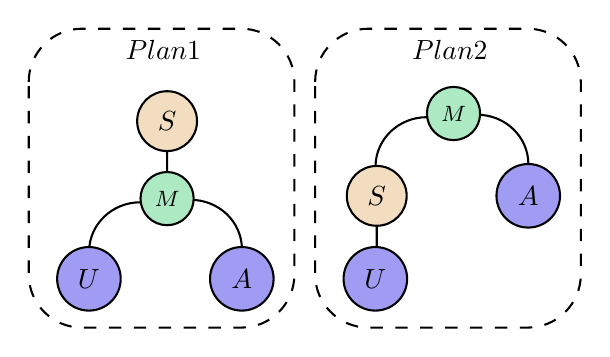
\begin{tikzpicture}[x=0.75pt,y=0.75pt,yscale=-1,xscale=1]
    %uncomment if require: \path (0,300); %set diagram left start at 0, and has height of 300
    
    %Rounded Rect [id:dp9327630093874044] 
    \draw  [dash pattern={on 4.5pt off 4.5pt}] (89,74.1) .. controls (89,59.96) and (100.46,48.5) .. (114.6,48.5) -- (191.4,48.5) .. controls (205.54,48.5) and (217,59.96) .. (217,74.1) -- (217,166.9) .. controls (217,181.04) and (205.54,192.5) .. (191.4,192.5) -- (114.6,192.5) .. controls (100.46,192.5) and (89,181.04) .. (89,166.9) -- cycle ;
    %Shape: Arc [id:dp8672386781469543] 
    \draw  [draw opacity=0] (118.09,155.74) .. controls (118.2,142.68) and (129.23,132.12) .. (142.82,132.12) -- (142.82,155.94) -- cycle ; \draw   (118.09,155.74) .. controls (118.2,142.68) and (129.23,132.12) .. (142.82,132.12) ;  
    %Shape: Arc [id:dp7960733152026014] 
    \draw  [draw opacity=0] (167,130.94) .. controls (180.66,130.94) and (191.73,141.6) .. (191.73,154.76) -- (167,154.76) -- cycle ; \draw   (167,130.94) .. controls (180.66,130.94) and (191.73,141.6) .. (191.73,154.76) ;  
    %Straight Lines [id:da6364636081987307] 
    \draw    (155.68,120.48) -- (155.67,107.08) ;
    
    
    %Rounded Rect [id:dp3039201957845239] 
    \draw  [dash pattern={on 4.5pt off 4.5pt}] (227,74.1) .. controls (227,59.96) and (238.46,48.5) .. (252.6,48.5) -- (329.4,48.5) .. controls (343.54,48.5) and (355,59.96) .. (355,74.1) -- (355,166.9) .. controls (355,181.04) and (343.54,192.5) .. (329.4,192.5) -- (252.6,192.5) .. controls (238.46,192.5) and (227,181.04) .. (227,166.9) -- cycle ;
    %Shape: Arc [id:dp6442642109452921] 
    \draw  [draw opacity=0] (256.09,114.74) .. controls (256.2,101.68) and (267.23,91.12) .. (280.82,91.12) -- (280.82,114.94) -- cycle ; \draw   (256.09,114.74) .. controls (256.2,101.68) and (267.23,91.12) .. (280.82,91.12) ;  
    %Shape: Arc [id:dp9997590238443537] 
    \draw  [draw opacity=0] (305,89.94) .. controls (305,89.94) and (305,89.94) .. (305,89.94) .. controls (318.66,89.94) and (329.73,100.6) .. (329.73,113.76) -- (305,113.76) -- cycle ; \draw   (305,89.94) .. controls (305,89.94) and (305,89.94) .. (305,89.94) .. controls (318.66,89.94) and (329.73,100.6) .. (329.73,113.76) ;  
    
    %Straight Lines [id:da7145621913901639] 
    \draw    (256.68,156.48) -- (256.67,143.08) ;

    % Text Node
    \draw  [fill={rgb, 255:red, 242; green, 221; blue, 192 }  ,fill opacity=1 ]  (155.67, 93.03) circle [x radius= 14.42, y radius= 14.42]   ;
    \draw (155.67,93.03) node    {$\text{S}$};
    % Text Node
    \draw  [fill={rgb, 255:red, 173; green, 234; blue, 195 }  ,fill opacity=1 ]  (155.67, 130.36) circle [x radius= 12.81, y radius= 12.81]   ;
    \draw (155.67,130.36) node  [font=\footnotesize]  {$\text{M}$};
    % Text Node
    \draw  [fill={rgb, 255:red, 160; green, 156; blue, 243 }  ,fill opacity=1 ]  (118.01, 169) circle [x radius= 15.31, y radius= 15.31]   ;
    \draw (118.01,169) node   [align=left] {$\displaystyle U$};
    % Text Node
    \draw  [fill={rgb, 255:red, 160; green, 156; blue, 243 }  ,fill opacity=1 ]  (191.67, 169) circle [x radius= 15.31, y radius= 15.31]   ;
    \draw (191.67,169) node   [align=left] {$\displaystyle A$};
    % Text Node
    \draw (134.17,52.73) node [anchor=north west][inner sep=0.75pt]    {$\text{Plan 1}$};
    % Text Node
    \draw  [fill={rgb, 255:red, 242; green, 221; blue, 192 }  ,fill opacity=1 ]  (256.67, 129.03) circle [x radius= 14.42, y radius= 14.42]   ;
    \draw (256.67,129.03) node    {$\text{S}$};
    % Text Node
    \draw  [fill={rgb, 255:red, 173; green, 234; blue, 195 }  ,fill opacity=1 ]  (293.67, 89.36) circle [x radius= 12.81, y radius= 12.81]   ;
    \draw (293.67,89.36) node  [font=\footnotesize]  {$\text{M}$};
    % Text Node
    \draw (272.17,52.73) node [anchor=north west][inner sep=0.75pt]    {$\text{Plan 2}$};
    % Text Node
    \draw  [fill={rgb, 255:red, 160; green, 156; blue, 243 }  ,fill opacity=1 ]  (256.01, 169) circle [x radius= 15.31, y radius= 15.31]   ;
    \draw (256.01,169) node   [align=left] {$\displaystyle U$};
    % Text Node
    \draw  [fill={rgb, 255:red, 160; green, 156; blue, 243 }  ,fill opacity=1 ]  (329.67, 129) circle [x radius= 15.31, y radius= 15.31]   ;
    \draw (329.67,129) node   [align=left] {$\displaystyle A$};
    
    
    \end{tikzpicture}
    \caption{Two example query plans for the sql query from figure \ref{figure:sql_query_example}.}
    \label{figure:example_query_plans}
\end{figure}

\newpage


In a large system that handles multiple requests per second, plans from different queries can have operations that are shared across. Combining these sub-sequences together can save additional execution time\cite{roy_multi-query_2009}. Finding the best combination of multiple queries and their plans has been proven to be an \emph{NP-Hard} problem\cite{sellis_multiple-query_1990}. This can be done classically with an exhaustive algorithm in $O(P^Q)$\footnote{as long as all queries have the same number of plans}, where $P$ is the number of plans and $Q$ the number of queries, as shown in figure \ref{figure:pseudocode_bruteforce_search}. The work of Kathurina et al.\cite{kathuria_provable_mqo} offers a greedy algorithm for finding a \emph{good} solution, whilst also proving that finding a better approximation factor for the greedy algorithm is \emph{NP-Hard}. A hybrid approach that combines classical and quantum computing uses QAOA (short for Quantum Approximate Optimization Algorithm)\cite{farhi_quantum_2014} have shown to be quasi-optimal solution finders with a runtime of $O(I \cdot (PQ)^2)$\cite{fankhauser_multiple_2021}. \par


\begin{listing}[!ht]
    \centering
    \begin{minted}{python}
        for plan_a in plans:
            for plan_b in plans:
                if plan_a.query != plan_b.query:
                    if savings(plan_a, plan_b) > current_savings:
                        current_savings = savings(plan_a, plan_b)
                        cheapest_combination = <plan_a, plan_b>
    \end{minted}
    \caption{Pseudocode of an exhaustive algorithm that tries every possible combination and finds the cheapest one.}
    \label{figure:pseudocode_bruteforce_search}
\end{listing}

 For example, if a second query that also filters the table $U$ for \code{USERS.NAME = "Abraham"} is supposed to run at roughly the same time, they could share a portion of the task. As shown in figure \ref{figure:example_query_plans}, the plans consist of multiple different instructions. Each instruction in any plan consist of single operations applied to tables of the database that are based on relational algebra\cite{codd_relational_1970}\footnote{But not limited to them, as modern databases also include hashing and indexing in the plans. Nonetheless, these operations can also be combined to save previous runtime}. 
 
 \newpage
 
 Figure \ref{figure:plan_tree} shows how the plans $\mathcal{Q}_0\mathcal{P}_0$ and $\mathcal{Q}_1\mathcal{P}_0$, from the differing queries $\mathcal{Q}_0$ and $\mathcal{Q}_1$, contain parts that can be reused, as shown in figure \ref{figure:plan_tree}. It is easy to imagine that, depending on the environment at hand, single operations will happen plenty of times in parallel. Putting into perspective the number of users that modern applications\cite{uber_technologies_inc_uber_2022} can have, finding shortcuts in plans does not only reduce execution time but saves money and improves customer experience.

\begin{figure}[!h]
    \centering
\tikzset{every picture/.style={line width=0.75pt}} %set default line width to 0.75pt        

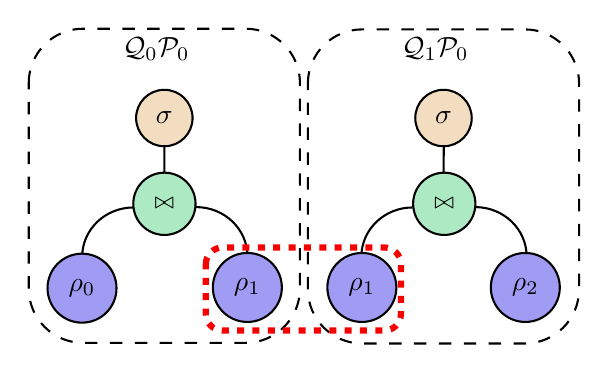
\begin{tikzpicture}[x=0.75pt,y=0.75pt,yscale=-1,xscale=1]
%uncomment if require: \path (0,300); %set diagram left start at 0, and has height of 300

%Rounded Rect [id:dp3098689700784747] 
\draw  [dash pattern={on 4.5pt off 4.5pt}] (120.33,155.05) .. controls (120.33,140.62) and (132.03,128.92) .. (146.47,128.92) -- (224.87,128.92) .. controls (239.3,128.92) and (251,140.62) .. (251,155.05) -- (251,254.12) .. controls (251,268.55) and (239.3,280.25) .. (224.87,280.25) -- (146.47,280.25) .. controls (132.03,280.25) and (120.33,268.55) .. (120.33,254.12) -- cycle ;
%Shape: Arc [id:dp8469571253916317] 
\draw  [draw opacity=0] (146.09,238.65) .. controls (146.2,225.59) and (157.23,215.04) .. (170.82,215.04) -- (170.82,238.86) -- cycle ; \draw   (146.09,238.65) .. controls (146.2,225.59) and (157.23,215.04) .. (170.82,215.04) ;  
%Shape: Arc [id:dp8173590455021038] 
\draw  [draw opacity=0] (201,214.86) .. controls (214.66,214.86) and (225.73,225.52) .. (225.73,238.67) -- (201,238.67) -- cycle ; \draw   (201,214.86) .. controls (214.66,214.86) and (225.73,225.52) .. (225.73,238.67) ;  
%Straight Lines [id:da6630213040029864] 
\draw    (185.68,199.4) -- (185.67,186) ;
%Rounded Rect [id:dp5436966787626745] 
\draw  [dash pattern={on 4.5pt off 4.5pt}] (254.83,155.38) .. controls (254.83,140.95) and (266.53,129.25) .. (280.97,129.25) -- (359.37,129.25) .. controls (373.8,129.25) and (385.5,140.95) .. (385.5,155.38) -- (385.5,254.45) .. controls (385.5,268.88) and (373.8,280.58) .. (359.37,280.58) -- (280.97,280.58) .. controls (266.53,280.58) and (254.83,268.88) .. (254.83,254.45) -- cycle ;
%Shape: Arc [id:dp13654717695684715] 
\draw  [draw opacity=0] (280.59,238.65) .. controls (280.7,225.59) and (291.73,215.04) .. (305.32,215.04) -- (305.32,238.86) -- cycle ; \draw   (280.59,238.65) .. controls (280.7,225.59) and (291.73,215.04) .. (305.32,215.04) ;  
%Shape: Arc [id:dp7676498647138272] 
\draw  [draw opacity=0] (335.5,214.86) .. controls (349.16,214.86) and (360.23,225.52) .. (360.23,238.67) -- (335.5,238.67) -- cycle ; \draw   (335.5,214.86) .. controls (349.16,214.86) and (360.23,225.52) .. (360.23,238.67) ;  
%Straight Lines [id:da7192788563309687] 
\draw    (320.18,199.4) -- (320.33,184.44) ;
%Rounded Rect [id:dp6770297453454031] 
\draw  [color={rgb, 255:red, 246; green, 1; blue, 1 }  ,draw opacity=1 ][dash pattern={on 2.53pt off 3.02pt}][line width=2.25]  (205.67,242.33) .. controls (205.67,237.92) and (209.25,234.33) .. (213.67,234.33) -- (291.67,234.33) .. controls (296.08,234.33) and (299.67,237.92) .. (299.67,242.33) -- (299.67,266.33) .. controls (299.67,270.75) and (296.08,274.33) .. (291.67,274.33) -- (213.67,274.33) .. controls (209.25,274.33) and (205.67,270.75) .. (205.67,266.33) -- cycle ;

% Text Node
\draw (164.17,131.65) node [anchor=north west][inner sep=0.75pt]    {$\mathcal{Q}_{0}\mathcal{P}_{0}$};
% Text Node
\draw  [fill={rgb, 255:red, 242; green, 221; blue, 192 }  ,fill opacity=1 ]  (185.67, 171.95) circle [x radius= 13.6, y radius= 13.6]   ;
\draw (185.67,171.95) node    {$\sigma $};
% Text Node
\draw (298.67,131.65) node [anchor=north west][inner sep=0.75pt]    {$\mathcal{Q}_{1}\mathcal{P}_{0}$};
% Text Node
\draw  [fill={rgb, 255:red, 242; green, 221; blue, 192 }  ,fill opacity=1 ]  (320.17, 171.95) circle [x radius= 13.6, y radius= 13.6]   ;
\draw (320.17,171.95) node    {$\sigma $};
% Text Node
\draw  [fill={rgb, 255:red, 173; green, 234; blue, 195 }  ,fill opacity=1 ]  (185.71, 213.28) circle [x radius= 15, y radius= 15]   ;
\draw (185.71,213.28) node  [font=\footnotesize]  {$\bowtie $};
% Text Node
\draw  [fill={rgb, 255:red, 173; green, 234; blue, 195 }  ,fill opacity=1 ]  (320.54, 213.28) circle [x radius= 15, y radius= 15]   ;
\draw (320.54,213.28) node  [font=\footnotesize]  {$\bowtie $};
% Text Node
\draw  [fill={rgb, 255:red, 160; green, 156; blue, 243 }  ,fill opacity=1 ]  (146.01, 253.92) circle [x radius= 16.62, y radius= 16.62]   ;
\draw (146.01,253.92) node   [align=left] {$\displaystyle \rho _{0}$};
% Text Node
\draw  [fill={rgb, 255:red, 160; green, 156; blue, 243 }  ,fill opacity=1 ]  (225.67, 253.58) circle [x radius= 16.62, y radius= 16.62]   ;
\draw (225.67,253.58) node   [align=left] {$\displaystyle \rho _{1}$};
% Text Node
\draw  [fill={rgb, 255:red, 160; green, 156; blue, 243 }  ,fill opacity=1 ]  (280.84, 253.58) circle [x radius= 16.62, y radius= 16.62]   ;
\draw (280.84,253.58) node   [align=left] {$\displaystyle \rho _{1}$};
% Text Node
\draw  [fill={rgb, 255:red, 160; green, 156; blue, 243 }  ,fill opacity=1 ]  (359.59, 253.58) circle [x radius= 16.62, y radius= 16.62]   ;
\draw (359.59,253.58) node   [align=left] {$\displaystyle \rho _{2}$};


\end{tikzpicture}


    \caption{Two differing plans $\mathcal{Q}_0\mathcal{P}_0$ and $\mathcal{Q}_1\mathcal{P}_1$, which serve different goals but contain the same operation $\rho_1$, marked in the red dotted box}
    \label{figure:plan_tree}
\end{figure}

Plans, costs, and savings can be mathematically expressed. Let there be given function $\mathcal{C}$ which returns the cost for a given operation or collection of operations, as defined in equation \ref{equation:formal_cost_function}. Let there also be a given function $\mathcal{S}$, which calculates the savings two collections of operations can achieve, as shown in equation \ref{equation:formal_savings_function}.

\begin{equation}
    \centering
    \begin{split}
        \mathcal{C}(\mathcal{Q}_0\mathcal{P}_1) =\ 45 \\
        \mathcal{C}(\rho_1) =\ 15 \\
    \end{split}
    \label{equation:formal_cost_function}
\end{equation}

\begin{equation}
    \centering
    \begin{split}
        \mathcal{S}(\mathcal{Q}_0\mathcal{P}_1, \mathcal{Q}_1\mathcal{P}_0) =\ 15 \\
        \mathcal{S}(\mathcal{Q}_0\mathcal{P}_0, \mathcal{Q}_1\mathcal{P}_1) =\ 0 \\
    \end{split}
    \label{equation:formal_savings_function}
\end{equation}


Taking a problem consisting of two queries $\mathcal{Q}_0$ and $\mathcal{Q}_1$, each of which has two plans $\mathcal{P}_0$ and $\mathcal{P}_1$, we can calculate the total costs of running them collectively as shown in equation \ref{equation:formal_total_cost_calculation}.

\begin{equation}
    \centering
    \begin{split}
        \mathcal{C}(\mathcal{Q}_0\mathcal{P}_0) + \mathcal{C}(\mathcal{Q}_1\mathcal{P}_0) - \mathcal{S}(\mathcal{Q}_0\mathcal{P}_0, \mathcal{Q}_1\mathcal{P}_0) \\
        \mathcal{C}(\mathcal{Q}_0\mathcal{P}_0) + \mathcal{C}(\mathcal{Q}_1\mathcal{P}_1) - \mathcal{S}(\mathcal{Q}_0\mathcal{P}_0, \mathcal{Q}_1\mathcal{P}_1) \\
        \mathcal{C}(\mathcal{Q}_0\mathcal{P}_1) + \mathcal{C}(\mathcal{Q}_1\mathcal{P}_0) - \mathcal{S}(\mathcal{Q}_0\mathcal{P}_1, \mathcal{Q}_1\mathcal{P}_0) \\
        \mathcal{C}(\mathcal{Q}_0\mathcal{P}_1) + \mathcal{C}(\mathcal{Q}_1\mathcal{P}_1) - \mathcal{S}(\mathcal{Q}_0\mathcal{P}_1, \mathcal{Q}_1\mathcal{P}_1) \\
    \end{split}
    \label{equation:formal_total_cost_calculation}
\end{equation}

If we change the problem space from two queries to more, or create an uneven number of plans per query, the complexity starts to rise sharply.


%%%%%%%%%%%%%%%%%%%%%%%%%%%%%%%%%%%%%%

\newpage

\section{Quantum Neural Network}

The \textit{classic computational neuron} originally proposed by Rosenblatt F.\cite{rosenblatt_perceptron_1958} as seen in figure \ref{figure:classic_computational_neuron} builds the bases for most neural networks used today. The underlying principle is simple, all inputs $x_n$ are multiplied by a weight $w_n$ and the sum is calculated. The calculated sum is passed to an activation function $f(x)$, which is activated if a predefined threshold value is exceeded. The activation function $f(x)$, also called transfer function, can be selected from a plethora of valid choices\cite{szandala_review_2021}

\tikzset{every picture/.style={line width=0.75pt}} %set default line width to 0.75pt        
\begin{figure}[h!]
    \centering

    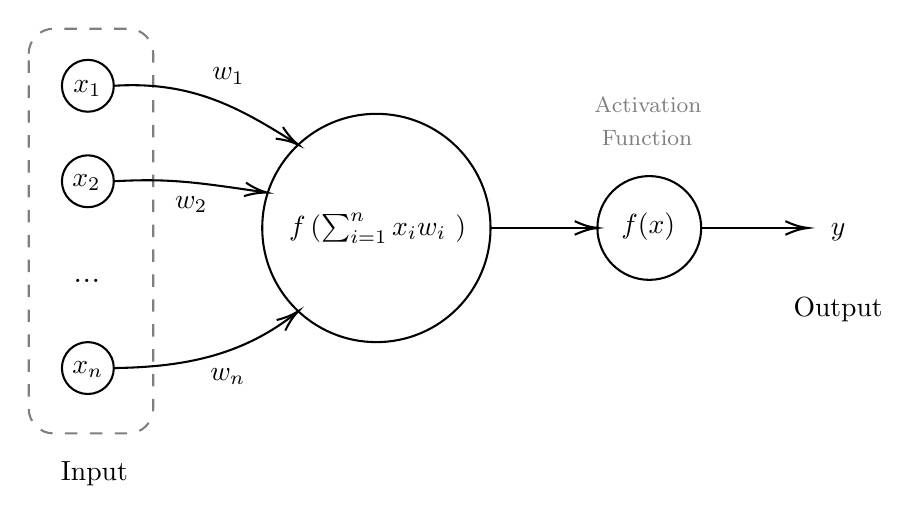
\begin{tikzpicture}[x=0.75pt,y=0.75pt,yscale=-1,xscale=1]
    %uncomment if require: \path (0,300); %set diagram left start at 0, and has height of 300
    
    %Shape: Circle [id:dp6859812572471455] 
    \draw   (192.5,140) .. controls (192.5,109.62) and (217.12,85) .. (247.5,85) .. controls (277.88,85) and (302.5,109.62) .. (302.5,140) .. controls (302.5,170.38) and (277.88,195) .. (247.5,195) .. controls (217.12,195) and (192.5,170.38) .. (192.5,140) -- cycle ;
    %Shape: Circle [id:dp24070647763127284] 
    \draw   (96,71.5) .. controls (96,64.6) and (101.6,59) .. (108.5,59) .. controls (115.4,59) and (121,64.6) .. (121,71.5) .. controls (121,78.4) and (115.4,84) .. (108.5,84) .. controls (101.6,84) and (96,78.4) .. (96,71.5) -- cycle ;
    %Shape: Circle [id:dp9363816782656273] 
    \draw   (96,117.5) .. controls (96,110.6) and (101.6,105) .. (108.5,105) .. controls (115.4,105) and (121,110.6) .. (121,117.5) .. controls (121,124.4) and (115.4,130) .. (108.5,130) .. controls (101.6,130) and (96,124.4) .. (96,117.5) -- cycle ;
    %Shape: Circle [id:dp4720861626805333] 
    \draw   (96,207.5) .. controls (96,200.6) and (101.6,195) .. (108.5,195) .. controls (115.4,195) and (121,200.6) .. (121,207.5) .. controls (121,214.4) and (115.4,220) .. (108.5,220) .. controls (101.6,220) and (96,214.4) .. (96,207.5) -- cycle ;
    %Rounded Rect [id:dp5631408345855224] 
    \draw  [color={rgb, 255:red, 0; green, 0; blue, 0 }  ,draw opacity=0.5 ][dash pattern={on 4.5pt off 4.5pt}] (80,56) .. controls (80,49.37) and (85.37,44) .. (92,44) -- (128,44) .. controls (134.63,44) and (140,49.37) .. (140,56) -- (140,227) .. controls (140,233.63) and (134.63,239) .. (128,239) -- (92,239) .. controls (85.37,239) and (80,233.63) .. (80,227) -- cycle ;
    %Curve Lines [id:da4059065253769214] 
    \draw    (121,71.5) .. controls (159.22,69.05) and (182.07,82.45) .. (208.38,98.98) ;
    \draw [shift={(210,100)}, rotate = 212.2] [color={rgb, 255:red, 0; green, 0; blue, 0 }  ][line width=0.75]    (10.93,-3.29) .. controls (6.95,-1.4) and (3.31,-0.3) .. (0,0) .. controls (3.31,0.3) and (6.95,1.4) .. (10.93,3.29)   ;
    %Curve Lines [id:da5094425475664381] 
    \draw    (121,207.5) .. controls (153.51,207.01) and (182.13,202.15) .. (208.78,180.98) ;
    \draw [shift={(210,180)}, rotate = 140.83] [color={rgb, 255:red, 0; green, 0; blue, 0 }  ][line width=0.75]    (10.93,-3.29) .. controls (6.95,-1.4) and (3.31,-0.3) .. (0,0) .. controls (3.31,0.3) and (6.95,1.4) .. (10.93,3.29)   ;
    %Curve Lines [id:da5523039314594727] 
    \draw    (121,117.5) .. controls (147.6,116.02) and (160.61,117.94) .. (193.48,122.78) ;
    \draw [shift={(195,123)}, rotate = 188.37] [color={rgb, 255:red, 0; green, 0; blue, 0 }  ][line width=0.75]    (10.93,-3.29) .. controls (6.95,-1.4) and (3.31,-0.3) .. (0,0) .. controls (3.31,0.3) and (6.95,1.4) .. (10.93,3.29)   ;
    %Straight Lines [id:da007343534667061169] 
    \draw    (302.5,140) -- (352,140) ;
    \draw [shift={(354,140)}, rotate = 180] [color={rgb, 255:red, 0; green, 0; blue, 0 }  ][line width=0.75]    (10.93,-3.29) .. controls (6.95,-1.4) and (3.31,-0.3) .. (0,0) .. controls (3.31,0.3) and (6.95,1.4) .. (10.93,3.29)   ;
    %Shape: Circle [id:dp683884067109112] 
    \draw   (354,140) .. controls (354,126.19) and (365.19,115) .. (379,115) .. controls (392.81,115) and (404,126.19) .. (404,140) .. controls (404,153.81) and (392.81,165) .. (379,165) .. controls (365.19,165) and (354,153.81) .. (354,140) -- cycle ;
    %Straight Lines [id:da9286309330170883] 
    \draw    (404,140) -- (453.5,140) ;
    \draw [shift={(455.5,140)}, rotate = 180] [color={rgb, 255:red, 0; green, 0; blue, 0 }  ][line width=0.75]    (10.93,-3.29) .. controls (6.95,-1.4) and (3.31,-0.3) .. (0,0) .. controls (3.31,0.3) and (6.95,1.4) .. (10.93,3.29)   ;
    
    % Text Node
    \draw (100,163) node [anchor=north west][inner sep=0.75pt]   [align=left] {{\large ...}};
    % Text Node
    \draw (100,67.4) node [anchor=north west][inner sep=0.75pt]    {$x_{1}$};
    % Text Node
    \draw (99.5,112.9) node [anchor=north west][inner sep=0.75pt]    {$x_{2}$};
    % Text Node
    \draw (99.5,202.9) node [anchor=north west][inner sep=0.75pt]    {$x_{n}$};
    % Text Node
    \draw (94,251) node [anchor=north west][inner sep=0.75pt]   [align=left] {Input};
    % Text Node
    \draw (167,61.4) node [anchor=north west][inner sep=0.75pt]    {$w_{1}$};
    % Text Node
    \draw (149,123.4) node [anchor=north west][inner sep=0.75pt]    {$w_{2}$};
    % Text Node
    \draw (166,206.4) node [anchor=north west][inner sep=0.75pt]    {$w_{n}$};
    % Text Node
    \draw (204,131.4) node [anchor=north west][inner sep=0.75pt]    {$f\left(\sum _{i=1}^{n} x_{i} w_{i} \ \right)$};
    % Text Node
    \draw (447,172) node [anchor=north west][inner sep=0.75pt]   [align=left] {Output};
    % Text Node
    \draw (364,131.4) node [anchor=north west][inner sep=0.75pt]    {$f( x)$};
    % Text Node
    \draw (465,136.4) node [anchor=north west][inner sep=0.75pt]    {$y$};
    % Text Node
    \draw (351,67) node [anchor=north west][inner sep=0.75pt]  [color={rgb, 255:red, 0; green, 0; blue, 0 }  ,opacity=0.5 ] [align=left] {\begin{minipage}[lt]{38.1pt}\setlength\topsep{0pt}
    \begin{center}
    {\footnotesize Activation}\\{\footnotesize Function}
    \end{center}
    
    \end{minipage}};
    
    \end{tikzpicture}

    \caption{Visual representation of the classic computational neuron, often referred to as a perceptron.}
    \label{figure:classic_computational_neuron}
\end{figure}

\begin{equation}
    \centering
    y =\ f\left(\sum_{i = 1}^n x_i\omega_i\right)
    \label{equation:classical_neuron_computation}
\end{equation}

\vspace{2em}
The quantum analogue of a classical neuron is called a quantum neuron also referred to as \textit{quron} as proposed by Maria Schuld et al. in their paper called "The quest for a Quantum Neural Network"\cite{schuldQuestQuantumNeural2014a}. ...


\subsection{Quantum Support Vector Machine (SVM)}
A classical support vector machine (SVM) also known as support vector network, initially conceived of by Cortes and Vapnik, divides a set of objects into classes in such a way that the widest possible area around the class boundaries remains free of objects. SVMs can not only perform linear classifications but also non-linear ones using the so-called kernel trick \cite{Cortes2004SupportVectorN}. A detailed explanation on how classical Support Vector Machines work can be found in the paper “Support vector machines explained” by Tristan Fletcher \cite{fletcher2009support}. 

Quantum SVM is considered to be the quantum analogue of the classical SVM algorithm as stated by Jiaying Yang et al. \cite{yangSupportVectorMachines2019}.

